\section{KHẢO SÁT SỰ BIẾN THIÊN VÀ VẼ ĐỒ THỊ HÀM SỐ}
\subsection{LÝ THUYẾT CẦN NHỚ}
\subsubsection{Sơ đồ khảo sát hàm số y= f(x)}
\begin{tcolorbox}[colframe=cyan,colback=red!3!white,boxrule=0.5mm]
		\begin{itemize}
		\item[\iconCH] \indamm{Bước 1.} Tìm tập xác định của hàm số.
		\item [\iconCH] \indamm{Bước 2.} Khảo sát sự biến thiên của hàm số
		\begin{itemize}
			\item Tính đạo hàm $y'$. Tìm các điểm mà tại đó $y'$ bằng $0$ hoặc đạo hàm không tồn tại.
			\item Tìm các giới hạn tại vô cực, giới hạn vô cực và tìm tiệm cận của đồ thị hàm số.
			\item Lập bảng biến thiên; xác định chiều biến thiên và cực trị của hàm số.
		\end{itemize}
		\item [\iconCH] \indamm{Bước 3.} Cho thêm điểm và vẽ đồ thị của hàm số dựa vào bảng biến thiên.
	\end{itemize}
\end{tcolorbox}
\subsubsection{Hàm số bậc ba $\mathbf{y=ax^3+bx^2+cx+d}$}
\	\begin{minipage}[b]{10cm}
		\begin{enumerate}[\iconCH]
			\item \indamm{TH1.} $y'=0$ có hai nghiệm phân biệt $x_1$ và $x_2$. Khi đó, hàm số có hai điểm cực trị $x=x_1$ và $x=x_2$.\\
			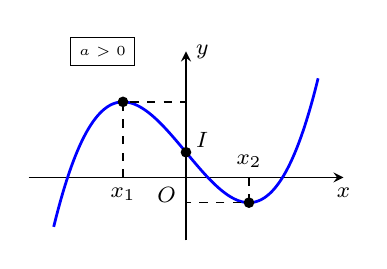
\begin{tikzpicture}[smooth,samples=300,line width=0.6pt,scale=0.8,>=stealth,font=\footnotesize]
				\draw[->] (-2.5,0)--(2.5,0) node[below]{$x$};
				\draw[->] (0,-1)--(0,2) node[right]{$y$};
				\draw (0,0) node[below left]{$O$};
				\draw[blue,line width=1pt,domain=-2.1:2.1] plot(\x,{0.4*((\x)^3-3*(\x)+1)});
				\draw[fill=black] (0,0.4) circle(2pt) (-1,1.2) circle(2pt) (1,-0.4) circle(2pt);
				\draw[dashed] (1,0)node[above]{\footnotesize$x_2$}--(1,-0.4)--(0,-0.4) (-1,0)node[below]{\footnotesize$x_1$}--(-1,1.2)--(0,1.2);
				\node[right] at (0,0.6) {\footnotesize $I$};
				\node[right] at (-2,2) {\tiny\fbox{$a>0$}};
			\end{tikzpicture}
			\hspace{0.3cm}
			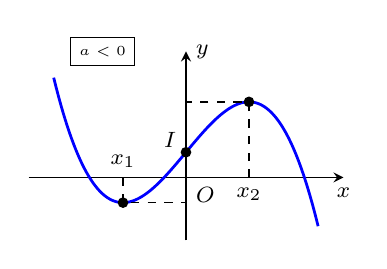
\begin{tikzpicture}[smooth,samples=300,line width=0.6pt,scale=0.8,>=stealth,font=\footnotesize]
				\draw[->] (-2.5,0)--(2.5,0) node[below]{$x$};
				\draw[->] (0,-1)--(0,2) node[right]{$y$};
				\draw (0,0) node[below right]{$O$};
				\draw[blue,line width=1pt,domain=-2.1:2.1] plot(\x,{0.4*(-(\x)^3+3*(\x)+1)});
				\draw[fill=black] (0,0.4) circle(2pt) (1,1.2) circle(2pt) (-1,-0.4) circle(2pt);
				\draw[dashed] (-1,0)node[above]{\footnotesize$x_1$}--(-1,-0.4)--(0,-0.4) (1,0)node[below]{\footnotesize$x_2$}--(1,1.2)--(0,1.2);
				\node[left] at (0,0.6) {\footnotesize$I$};
				\node[right] at (-2,2) {\tiny\fbox{$a<0$}};
			\end{tikzpicture}
			\item \indamm{TH2.} $y'=0$ có nghiệm kép $x_0$. Khi đó, hàm số không có cực trị.\\
			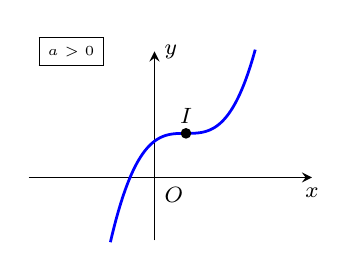
\begin{tikzpicture}[smooth,samples=300,line width=0.6pt,scale=0.8,>=stealth,font=\footnotesize]
				\draw[->] (-2,0)--(2.5,0) node[below]{$x$};
				\draw[->] (0,-1)--(0,2) node[right]{$y$};
				\draw (0,0) node[below right]{$O$};
				\draw[blue,line width=1pt,domain=-0.7:1.6] plot(\x,{(\x-0.5)^3+0.7});
				\draw[fill=black] (0.5,0.7) circle(2pt);
				\node[above] at (0.5,0.7) {\footnotesize$I$};
				\node[right] at (-2,2) {\tiny\fbox{$a>0$}};
			\end{tikzpicture}
			\hspace{0.5cm}
			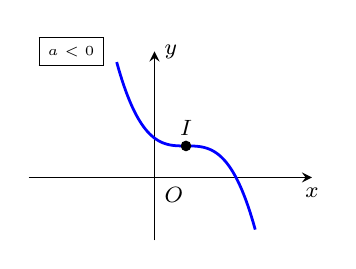
\begin{tikzpicture}[smooth,samples=300,line width=0.6pt,scale=0.8,>=stealth,font=\footnotesize]
				\draw[->] (-2,0)--(2.5,0) node[below]{$x$};
				\draw[->] (0,-1)--(0,2) node[right]{$y$};
				\draw (0,0) node[below right]{$O$};
				\draw[blue,line width=1pt,domain=-0.6:1.6] plot(\x,{-((\x-0.5)^3-0.5)});
				\draw[fill=black] (0.5,0.5) circle(2pt);
				\node[above] at (0.5,0.5) {\footnotesize$I$};
				\node[right] at (-2,2) {\tiny\fbox{$a<0$}};
			\end{tikzpicture}
			\item \indamm{TH3.} $y'=0$ vô nghiệm. Khi đó, hàm số không có cực trị.\\
			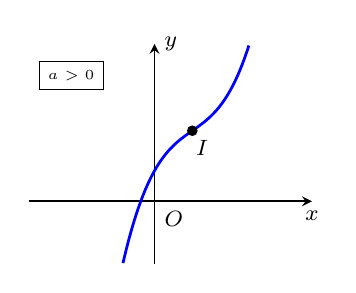
\begin{tikzpicture}[smooth,samples=300,line width=0.6pt,scale=0.8,>=stealth,font=\footnotesize]
				\draw[->] (-2,0)--(2.5,0) node[below]{$x$};
				\draw[->] (0,-1)--(0,2.5) node[right]{$y$};
				\draw (0,0) node[below right]{$O$};
				\draw[blue,line width=1pt,domain=-0.5:1.5] plot(\x,{((\x-0.6)^3+0.7*(\x)+0.7)});
				\draw[fill=black] (0.6,1.12) circle(2pt);
				\node[below right] at (0.5,1.12) {\footnotesize$I$};
				\node[right] at (-2,2) {\tiny\fbox{$a>0$}};
			\end{tikzpicture}
			\hspace{0.5cm}
			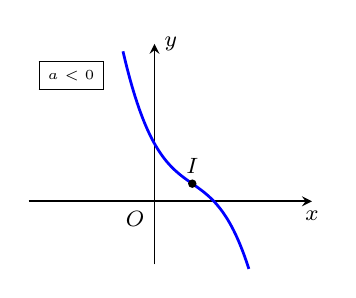
\begin{tikzpicture}[smooth,samples=300,line width=0.6pt,scale=0.8,>=stealth,font=\footnotesize]
				\draw[->] (-2,0)--(2.5,0) node[below]{$x$};
				\draw[->] (0,-1)--(0,2.5) node[right]{$y$};
				\draw (0,0) node[below left]{$O$};
				\draw[blue,line width=1pt,domain=-0.5:1.5] plot(\x,{-(\x-0.6)^3-0.7*(\x)+0.7)});
				\draw[fill=black] (0.6,0.28) circle(1.5pt);
				\node[right] at (-2,2) {\tiny\fbox{$a<0$}};
				\node[above] at (0.6,0.28) {\footnotesize$I$};
			\end{tikzpicture}
		\end{enumerate}
		\vspace{0.4cm}
	\end{minipage}\hspace{0.5cm}
	\begin{minipage}[b]{6.5cm}
		\begin{khung4}{GHI NHỚ}
			\ding{172} Hàm số không có điểm cực trị
			$$b^2-3ac\le 0 \text{ hoặc } \heva{&a=0 \\&b=0.}$$
			\ding{173} Hàm số có hai điểm cực trị
			$$\heva{&a \ne 0\\&b^2-3ac >0.}$$
			\ding{174} Liên hệ tổng tích hai nghiệm
			$$\heva{&x_1+x_2=-\dfrac{2b}{3a}\\&x_1x_2=\dfrac{c}{3a}}$$
			\ding{175} Tọa độ tâm đối xứng của đồ thị, nó chính là trung điểm của đoạn nối 2 điểm cực trị. Hoành độ tâm đối xứng là nghiệm phương trình $y''=0 \Leftrightarrow x=-\dfrac{b}{3a}$.
			\ding{176} Tiếp tuyến tại tâm đối xứng sẽ có hệ số góc nhỏ nhất nếu $a>0$ và lớn nhất nếu $a<0$.
		\end{khung4}
		\vspace{0.1cm}
	\end{minipage}
\newpage
\subsubsection{Hàm số $\mathbf{y = \dfrac{{ax + b}}{{cx + d}}\left( {c \ne 0,ad - bc \ne 0} \right)}$}
\begin{minipage}[b]{10cm}
	\begin{enumerate}[\iconCH]
		\item Tập xác định $D=\mathbb{R}\backslash \left\{-\dfrac{d}{c}\right\}$; Đạo hàm $y'=\dfrac{ad-cb}{(cx+d)^2}$.
		\item Đồ thị nhận giao điểm của hai đường tiệm cận làm tâm đối xứng.
		\item Hình dạng đồ thị:\\
		\begin{tikzpicture}[smooth,samples=300,line width=0.6pt,>=stealth, scale=0.45]
			\draw[->] (-5,0)--(3.5,0) node[below]{$x$};
			\draw[->] (0,-1.6)--(0,5.7) node[right]{$y$};
			\draw (0,0) node[below right]{$O$};
			\node at (-3,5.3) {\tiny\fbox{$y'>0$}};
			\clip (-5,-1.5) rectangle (3,5.5);
			\draw[dashed] (-1,-2)--(-1,5.5) (-5,2)--(3,2);
			\draw[blue,line width=1pt,domain=-5:-1.1] plot(\x,{(2*(\x)+1)/((\x)+1)});
			\draw[blue,line width=1pt,domain=-0.9:3] plot(\x,{(2*(\x)+1)/((\x)+1)});
			\draw[fill=black] (-1,2) circle(1.5pt) circle(1.5pt) (-1,0) circle(1pt) (0,2) circle(1pt);
			\node[left] at (-1,1.5) {\footnotesize $I$};
			\node[below left] at (-1,0) {\tiny $-\dfrac{d}{c}$};
			\node[above right] at (0,2) {\tiny $\dfrac{a}{c}$};
		\end{tikzpicture}
		\hspace{0.5cm}
		\begin{tikzpicture}[smooth,samples=300,line width=0.6pt,>=stealth, scale=0.45]
			\draw[->] (-3,0)--(5.5,0) node[below]{$x$};
			\draw[->] (0,-1.6)--(0,5.7) node[left]{$y$};
			\draw (0,0) node[below left]{$O$};
			\node at (3,5.3) {\tiny \fbox{$y'<0$}};
			\clip (-3,-1.5) rectangle (5,5.5);
			\draw[dashed] (1,-2)--(1,5.5) (-3,2)--(5,2);
			\draw[blue,line width=1pt,domain=-3:0.9] plot(\x,{(2*(\x)-1)/((\x)-1)});
			\draw[blue,line width=1pt,domain=1.1:5] plot(\x,{(2*(\x)-1)/((\x)-1)});
			\draw[fill=black] (1,2) circle(1.5pt) (1,0) circle(1pt) (0,2) circle(1pt);
			\node[right] at (1,1.5) {\footnotesize $I$};
			\node[below right] at (1,0) {\tiny $-\dfrac{d}{c}$};
			\node[above left] at (0,2) {\tiny $\dfrac{a}{c}$};
		\end{tikzpicture}
	\end{enumerate}
	%	\vspace{1.5cm}
\end{minipage}\hspace{0.5cm}
\begin{minipage}[b]{6.5cm}
	\begin{khung4}{GHI NHỚ}
		\ding{172} Tiệm cận đứng $x=-\dfrac{d}{c}$.\\
		\ding{173} Tiệm cận ngang $y=\dfrac{a}{c}$.\\
		\ding{174} Giao với $Ox$: $y=0 \Rightarrow x=-\dfrac{b}{a}$.\\
		\ding{175} Giao với $Oy$: $x=0 \Rightarrow y=\dfrac{b}{d}$.\\
	\end{khung4}
\end{minipage}
\subsubsection{Hàm số $\mathbf{y = \dfrac{{a{x^2} + bx + c}}{{mx + n}}\left( {a \ne 0,m \ne 0} \right)}$ (đa thức tử không chia hết cho đa thức mẫu)}
\begin{enumerate}[\iconCH]
	\item Tập xác định $D=\mathbb{R}\backslash \left\{-\dfrac{n}{m}\right\}$; Đạo hàm $y'=\dfrac{am\cdot x^2+2an\cdot x + b.n - m.c}{(mx+n)^2}$.
	\item Hàm số $2$ điểm cực trị khi $y'=0$ có $2$ nghiệm phân biệt; Hàm số không có cực trị khi $y'=0$ vô nghiệm.
	\item Đồ thị nhận giao điểm của tiệm cận đứng và tiệm cận xiên làm tâm đối xứng.
	\item Hình dạng đồ thị:\\
	\begin{tikzpicture}[line cap=butt,line join=miter,>=stealth,scale=0.4,font=\footnotesize]
		\tikzset{declare function={xmin=-5.5;xmax=3.5;ymin=-4.6;ymax=4.6;},
			smooth,samples=450}
		\draw[->] (xmin,-0.5)--(xmax,-0.5) node[above]{$ x $};
		\draw[->] (0,ymin)--(0,ymax) node[right]{$ y $};
		\fill (0,-0.5) node[above right]{$ O $};
		\path (current bounding box.south) node[below, black]{\tiny\fbox{$a>0$, $y'=0$ có $2$ nghiệm phân biệt}};
		\clip (xmin,ymin) rectangle (xmax,ymax);
		\def\f(#1){((#1)^2+2*(#1)+2)/((#1)+1)} % Hàm số
		\def\q(#1){((#1)+1)} % Tiệm cận xiên	
		\draw[blue,thick,samples=250] plot[domain=xmin:-1.1] (\x,{\f(\x)});	
		\draw[blue,thick,samples=250] plot[domain=-0.9:xmax] (\x,{\f(\x)});
		%--------- Tiệm cận
		\draw[dashed] plot [domain=xmin:xmax] (\x,{\q(\x)}) ;
		\draw[dashed] (-1,ymin)--(-1,ymax);
	\end{tikzpicture}	
	\hspace{.25cm}
	\begin{tikzpicture}[line cap=butt,line join=miter,>=stealth,scale=0.4,font=\footnotesize]
		\tikzset{declare function={xmin=-5.5;xmax=3.5;ymin=-4.6;ymax=4.6;},
			smooth,samples=450}
		\draw[->] (xmin,-0.5)--(xmax,-0.5) node[above]{$ x $};
		\draw[->] (0,ymin)--(0,ymax) node[right]{$ y $};
		\fill (0,-0.5) node[above right]{$ O $};
		\path (current bounding box.south) node[below, black]{\tiny\fbox{$a<0$, $y'=0$ có $2$ nghiệm phân biệt}};
		\clip (xmin,ymin) rectangle (xmax,ymax);
		\def\f(#1){(-(#1)^2-2*(#1)-2)/((#1)+1)} % Hàm số
		\def\q(#1){(-(#1)-1)} % Tiệm cận xiên	
		\draw[blue,thick,samples=250] plot[domain=xmin:-1.1] (\x,{\f(\x)});	
		\draw[blue,thick,samples=250] plot[domain=-0.9:xmax] (\x,{\f(\x)});
		%--------- Tiệm cận
		\draw[dashed] plot [domain=xmin:xmax] (\x,{\q(\x)}) ;
		\draw[dashed] (-1,ymin)--(-1,ymax);
	\end{tikzpicture}	
	\hspace{.25cm}
	\begin{tikzpicture}[line cap=butt,line join=miter,>=stealth,scale=0.4,font=\footnotesize]
		\tikzset{declare function={xmin=-5.5;xmax=3.5;ymin=-4.6;ymax=4.6;},
			smooth,samples=450}
		\draw[->] (xmin,-0.5)--(xmax,-0.5) node[above]{$ x $};
		\draw[->] (0,ymin)--(0,ymax) node[right]{$ y $};
		\fill (0,-0.5) node[above right]{$ O $};
		\path (current bounding box.south) node[below, black]{\tiny\fbox{$a>0$, $y'=0$ vô nghiệm}};
		\clip (xmin,ymin) rectangle (xmax,ymax);
		\def\f(#1){((#1)^2+2*(#1))/((#1)+1)} % Hàm số
		\def\q(#1){((#1)+1)} % Tiệm cận xiên	
		\draw[blue,thick,samples=250] plot[domain=xmin:-1.1] (\x,{\f(\x)});	
		\draw[blue,thick,samples=250] plot[domain=-0.9:xmax] (\x,{\f(\x)});
		%--------- Tiệm cận
		\draw[dashed] plot [domain=xmin:xmax] (\x,{\q(\x)}) ;
		\draw[dashed] (-1,ymin)--(-1,ymax);
	\end{tikzpicture}	
	\hspace{.25cm}
	\begin{tikzpicture}[line cap=butt,line join=miter,>=stealth,scale=0.4,font=\footnotesize]
		\tikzset{declare function={xmin=-5.5;xmax=3.5;ymin=-4.6;ymax=4.6;},
			smooth,samples=450}
		\draw[->] (xmin,-0.5)--(xmax,-0.5) node[above]{$ x $};
		\draw[->] (0,ymin)--(0,ymax) node[right]{$ y $};
		\fill (0,-0.5) node[above right]{$ O $};
		\path (current bounding box.south) node[below, black]{\tiny\fbox{$a<0$, $y'=0$ vô nghiệm}};
		\clip (xmin,ymin) rectangle (xmax,ymax);
		\def\f(#1){(-(#1)^2-2*(#1))/((#1)+1)} % Hàm số
		\def\q(#1){(-(#1)-1)} % Tiệm cận xiên	
		\draw[blue,thick,samples=250] plot[domain=xmin:-1.1] (\x,{\f(\x)});	
		\draw[blue,thick,samples=250] plot[domain=-0.9:xmax] (\x,{\f(\x)});
		%--------- Tiệm cận
		\draw[dashed] plot [domain=xmin:xmax] (\x,{\q(\x)}) ;
		\draw[dashed] (-1,ymin)--(-1,ymax);
	\end{tikzpicture}
\end{enumerate}
\subsection{PHÂN LOẠI VÀ PHƯƠNG PHÁP GIẢI TOÁN}
\begin{dang}{Khảo sát và vẽ đồ thị hàm số bậc ba}
	Ta khảo sát theo sơ đồ đã nhắc đến ở phần lý thuyết.
\end{dang}
\boxmini{BÀI TẬP TỰ LUẬN}
\begin{vd}
	Khảo sát sự biến thiên và vẽ đồ thị các hàm số sau:
	\begin{tasks}(2)
		\task $y=x^3-3x^2+1$;
		\task $y =-2{x^3}-3{x^2}+1$;
		\task $y = {x^3}+3{x^2}+3x+2$;
		\task $y=x^3-3x^2+4x-2$.
	\end{tasks}
\loigiai{
\begin{enumerate}[a)]
	\item Tập xác định $\mathbb{R}$.\\
	Sự biến thiên:
	\begin{itemize}
		\item [$\bullet$] $y'=3x^2-6x$; $y'=0\Leftrightarrow \hoac{&x=0\\&x=2.}$.
		\item [$\bullet$]  Giới hạn: $\lim\limits_{x\to -\infty}y=-\infty$; $\lim\limits_{x\to +\infty}y=+\infty$.
		\item [$\bullet$] \immini{Bảng biến thiên như hình bên:\\
		Suy ra hàm số đồng biến trên các khoảng $(-\infty;0)$ và $(2;+\infty)$; nghịch biến trên $(0;2)$.\\
	Hàm số đạt cực đại tại $x=0; y_{\text{CĐ}}=1$; hàm số đạt cực tiểu tại $x=2; y_{\text{CT}}=-3$.}
	{\hspace{1cm}
		
\begin{tikzpicture}
			\tkzTabInit[lgt=1.1,espcl=2,nocadre=True]{$x$/0.6,$y'$/0.6,$y$/2}{$-\infty$,$0$,$2$,$+\infty$}
			\tkzTabLine{,+,z,-,z,+,}
			\tkzTabVar{-/$-\infty$ , +/$1$,-/$-3$, +/$+\infty$}%
		\end{tikzpicture}}
			\end{itemize}
		Đồ thị:
			\immini{
				\begin{itemize}
					\item [$\bullet$] Đồ thị đi qua các điểm $(2;-3)$, $(-1;-3)$, $(3;1)$
					\item [$\bullet$] Đồ thị nhận điểm $I(1;-1)$ làm tâm đối xứng.
				\end{itemize}
				}
			{
				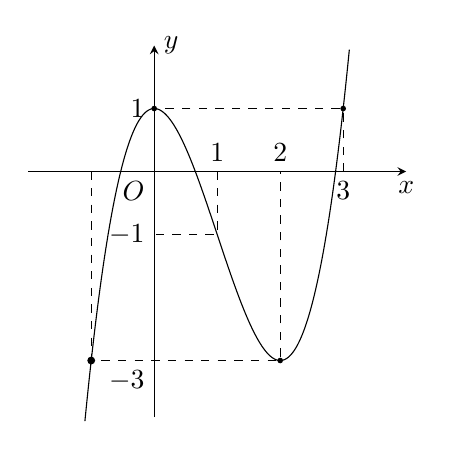
\begin{tikzpicture}[smooth,samples=300,scale=0.8,>=stealth]
					\draw[->] (-2,0)--(4,0) node[below]{$x$};
					\draw[->] (0,-3.9)--(0,2) node[right]{$y$};
					\draw (0,0) node[below left]{$O$};
					\draw[domain=-1.1:3.1] plot(\x,{(\x)^3-3*(\x)^2+1});
					\draw[fill=black] (-1,-3) circle(1.5pt) (0,1) circle(1pt) (2,-3) circle(1pt) (3,1) circle(1pt);
					\draw[dashed] (-1,0)--(-1,-3)--(0,-3)node[below left]{$-3$}--(2,-3)--(2,0)node[above]{$2$}
					(1,0)node[above]{$1$}--(1,-1)--(0,-1)node[left]{$-1$}
					(3,0)node[below]{$3$}--(3,1)--(0,1)node[left]{$1$}
					;
				\end{tikzpicture}
			}
	\item Tập xác định: $\mathbb{R}$.\\
	Sự biến thiên:
	\begin{itemize}
		\item [$\bullet$] $y' = - 6{x^2} - 6x;\,\,y' = 0 \Leftrightarrow x = 0$ hoặc $x = - 1$.
		\item [$\bullet$]  Giới hạn: $\lim\limits_{x\to -\infty}y=+\infty$; $\lim\limits_{x\to +\infty}y=-\infty$.
		\item [$\bullet$] \immini{Bảng biến thiên như hình bên:\\
			Suy ra hàm số nghịch biến trên các khoảng $(-\infty;-1)$ và $(0;+\infty)$; đồng biến trên $(-1;0)$.\\
			Hàm số đạt cực đại tại $x=0; y_{\text{CĐ}}=1$; hàm số đạt cực tiểu tại $x=-1; y_{\text{CT}}=0$.}
		{\hspace{1cm}
			
\begin{tikzpicture}[scale=1, font=\footnotesize, line join=round, line cap=round, >=stealth]
				\tkzTabInit[nocadre=false,lgt=1.2,espcl=1.6,deltacl=0.6]
				{$x$ /0.6,$f'(x)$ /0.6,$f(x)$ /1.5}
				{$-\infty$,$-1$,$0$,$+\infty$}
				\tkzTabLine{,-,0,+,0,-,}
				\tkzTabVar{+/$+\infty$,-/$0$,+/$1$,-/$-\infty$}
		\end{tikzpicture}}
	\end{itemize}
Đồ thị:
	\immini{
		\begin{itemize}
			\item [$\bullet$] Đồ thị qua các điểm $(1;-4)$, $(-2;5)$.
			\item [$\bullet$] Đồ thị của hàm số có tâm đối xứng là điểm $I\left({- \dfrac{1}{2};\dfrac{1}{2}} \right)$
		\end{itemize}
		}{	
		\begin{tikzpicture}[scale=1.0,>=stealth, font=\footnotesize, line join=round, line cap=round]
			\def\xmin{-2} \def\xmax{2}
			\def\ymin{-2} \def\ymax{2}
			\draw[->] (\xmin,0)--(\xmax,0) node [below]{$x$};
			\draw[->] (0,\ymin)--(0,\ymax) node [left]{$y$};
			\fill (0,0) circle (1pt) node[shift={(-135:2.5mm)}]{$O$};
			\clip (\xmin+0.1,\ymin+0.1) rectangle (\xmax-0.1,\ymax-0.1);
			\draw[smooth,red,samples=300,domain=(\xmin:3.01)] plot(\x,{-2*(\x)^3-3*(\x)^2+1});	
			\foreach \x in {\xmin,...,\xmax}
			\draw (\x,-0.05)--(\x,0.05);
			\foreach \y in {\ymin,...,\ymax}
			\draw (-0.05,\y)--(0.05,\y);
			\node at (-1,0)[below]{$ -1 $};
			\node at (1,0)[below]{$ 1 $};	
			\node at (0,1)[shift={(135:1.5mm)}]{$ 1 $};	
	\end{tikzpicture}}
	\item Tập xác định $\mathbb{R}$.\\
	Sự biến thiên:
	\begin{itemize}
		\item [$\bullet$] $y' = 3{x^2} + 6x + 3;\,\,y' = 0 \Leftrightarrow x = - 1$.
		\item [$\bullet$] Giới hạn: $\lim\limits_{x\to -\infty}y=-\infty$; $\lim\limits_{x\to +\infty}y=+\infty$.
		\item [$\bullet$] \immini{Bảng biến thiên như hình bên:\\
			Suy ra hàm số đồng biến trên $\mathbb{R}$.\\
			Hàm số không có cực trị.}
		{\hspace{1cm}
			
\begin{tikzpicture}[>=stealth]
				\tkzTabInit[nocadre=false,lgt=1,espcl=2.5,deltacl=0.5]{$x$/.6 ,$y'$/.6,$y$/1.5}
				{$-\infty$ , $-1$ , $+\infty$}
				\tkzTabLine{ , + , $0$ , + , }
				\tkzTabVar{-/$-\infty$ , R , +/$+\infty$}
				\tkzTabIma{1}{3}{2}{$1$}
		\end{tikzpicture}}
	\end{itemize}
	Đồ thị:
		\immini{	
	Đồ thị của hàm số có tâm đối xứng là điểm $I\left( {- 1;1} \right)$
	}{	
		\begin{tikzpicture}[scale=0.7,>=stealth, font=\footnotesize, line join=round, line cap=round]
			\def\xmin{-3} \def\xmax{2}
			\def\ymin{-2} \def\ymax{4}
			\draw[->] (\xmin,0)--(\xmax,0) node [below]{$x$};
			\draw[->] (0,\ymin)--(0,\ymax) node [left]{$y$};
			\fill (0,0) circle (1pt) node[shift={(-135:2.5mm)}]{$O$};
			\clip (\xmin+0.1,\ymin+0.1) rectangle (\xmax-0.1,\ymax-0.1);
			\draw[smooth,red,samples=300,domain=(\xmin:3.01)] plot(\x,{(\x)^3+3*(\x)^2+3*(\x)+2});	
			\foreach \x in {\xmin,...,\xmax}
			\draw (\x,-0.05)--(\x,0.05);
			\foreach \y in {\ymin,...,\ymax}
			\draw (-0.05,\y)--(0.05,\y);	
			\node at (1,0)[below]{$ 1 $};
			\node at (-1,1)[shift={(70:2mm)}]{$ I $};
			\draw[dashed]
			(-1,0)node[below]{$ -1 $}|-(0,1)node[right]{$1$}	
			;	
		\end{tikzpicture}}				
	\item Tập xác định: $\mathbb{R}$.\\
	Sự biến thiên
	\begin{itemize}
		\item [$\bullet$] $y'=3x^2-6x+4>0$ với $\forall x\in\mathbb{R}$.
		\item [$\bullet$] Giới hạn: $\lim\limits_{x\to -\infty}y=-\infty$; $\lim\limits_{x\to +\infty}y=+\infty$
		\item [$\bullet$] \immini{Bảng biến thiên như hình bên:\\
			Suy ra hàm số đồng biến trên $\mathbb{R}$.\\
			Hàm số không có cực trị.}
		{\hspace{1cm}
			
\begin{tikzpicture}
				\tkzTabInit[lgt=1.1,espcl=4]{$x$/0.6,$y'$/0.6,$y$/2}{$-\infty$,$+\infty$}
				\tkzTabLine{,+,}
				\tkzTabVar{-/$-\infty$ ,+/$+\infty$}
		\end{tikzpicture}}
	\end{itemize}
Đồ thị\\
\immini{
	\begin{itemize}
		\item [$\bullet$] Đồ thị đi qua $(2;2)$, $(0;-2)$, $(1;0)$.
		\item [$\bullet$] Đồ thị nhận $I(1;0)$ làm tâm đối xứng.
	\end{itemize}
}
{
	\begin{tikzpicture}[line cap=round,line join=round,x=1cm,y=1cm]
		\draw[->](-3.08,0)--(4.06,0);
		\foreach \x in {-1,2,3}
		\draw[shift={(\x,0)},color=black] (0pt,2pt)--(0pt,-2pt) node[below]{$\x$};
		\draw[->,color=black](0,-4.06)--(0,2.98);
		\foreach \y in {-2,-1,1,2}
		\draw[shift={(0,\y)},color=black](2pt,0pt)--(-2pt,0pt) node[left]{\normalsize $\y$};
		\draw[color=black](3.8,.2)node[right]{$x$};
		\draw[color=black](.2,3)node[right]{$y$};
		\draw[color=black](0pt,-8pt)node[right]{\normalsize $O$};
		\clip(-3.08,-4.06) rectangle (4.06,2.98);
		%Vẽ đồ thị
		\draw[smooth,samples=100,domain=-4:4]plot(\x,{(\x)^3-3*(\x)^2+4*(\x)-2});
		%Vẽ râu ria
		\draw[dashed](2,0)--(2,2)--(0,2);
		\node[below right] at (1,0){$I$};
		\node[above] at (1,0) {$1$};
	\end{tikzpicture}
}
\end{enumerate}
}
\end{vd}
\dongcham{45}
\boxmini{BÀI TẬP TRẮC NGHIỆM}
\ind{PHẦN I.} \inden{Câu trắc nghiệm nhiều phương án lựa chọn. Mỗi câu hỏi học sinh chỉ chọn một phương án.}\\
\setcounter{ex}{0}
\Opensolutionfile{ans}[ans/2D1-B4-d1-1]
\begin{ex}
	\immini[thm]{Bảng biến thiên ở hình bên là của một trong bốn hàm số sau đây. Hỏi đó là hàm số nào?
		\choice
		{$y=-x^3-2x^2+5$}
		{\True $y=x^3-3x^2+5$}
		{$y=-x^3-3x+5$}
		{$y=x^3+3x^2+5$}}{
		
\begin{tikzpicture}
			\tkzTabInit[nocadre=false, lgt=1.2, espcl=1.6]{$x$ /0.6,$f'(x)$ /0.6,$f(x)$ /1.5}{$-\infty$,$0$,$2$,$+\infty$}
			\tkzTabLine{,+,$0$,-,$0$,+,}
			\tkzTabVar{-/ $-\infty$/, +/$5$ , -/$1$  , +/$+\infty$/}
	\end{tikzpicture}}
\end{ex} \dongcham{1}

\begin{ex}
	\immini[thm]{Bảng biến thiên ở hình bên là của một trong bốn hàm số sau đây. Hỏi đó là hàm số nào?
	\choice
	{$ y=-x^3+3x^2 $}
	{$ y=x^3-3x^2-1$}
	{$ y=x^4+2x^2+1 $}
	{\True$ y=-x^3+3x^2+1 $}}{

\begin{tikzpicture}
	\tkzTabInit[nocadre=false,lgt=1.2,espcl=1.6,deltacl=0.6]
	{$x$/0.6, $y'$/0.6, $y$/1.5}
	{$-\infty$,$0$,$2$,$+\infty$}
	\tkzTabLine{,-,z,+,z,-,}
	\tkzTabVar{+/$+\infty$ ,-/ $1$ ,+/$5$, -/$-\infty$}
\end{tikzpicture}}
	\loigiai{
		Ta thấy đây là hàm số bậc ba và $\displaystyle\lim\limits_{x\rightarrow-\infty}=-\infty$ nên $a<0$.\\
		Ta có $f(0)=1$ nên hàm số cần tìm là $y=-x^3+3x^2+1$.
	}
\end{ex} \dongcham{1}

\begin{ex}
	\immini[thm]{Bảng biến thiên ở hình bên là của một trong bốn hàm số sau đây. Hỏi đó là hàm số nào?
		\haicot
		{$y=x^3-3x^2+x+3$}
		{$y=x^3-3x+4$}
		{\True $y=x^3-3x^2+3x+1$}
		{$y=x^3+3x^2+5$}}{
		
\begin{tikzpicture}
			\tkzTabInit[lgt=1,espcl=2.5]
			{$x$/0.6,$y'$/0.6,$y$/1.5}
			{$-\infty$,$1$,$+\infty$}
			\tkzTabLine{,+,$0$,+,}
			\tkzTabVar{-/$-\infty$,R,+/$+\infty$}
			\tkzTabIma[draw]{1}{3}{2}{$2$}
	\end{tikzpicture}}
\end{ex} \dongcham{1}

\begin{ex}%[2D1B5-1]
	\immini[thm]{Đường cong bên là đồ thị của một trong bốn hàm số đã cho sau đây. Hỏi đó là hàm số nào?
		\choice
		{$y=-x^3+x^2-2$}
		{\True $y=x^3+3x^2-2$}
		{$y=x^3-3x+2$}
		{$y=x^2-3x-2$}
	}{
		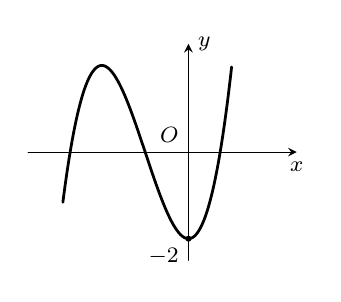
\begin{tikzpicture}[scale=0.55, font=\footnotesize,line join=round, line cap=round,>=stealth]
			\draw[->] (-3.7,0.) -- (2.5,0.) node[below]{$x$};
			\draw[->] (0,-2.5) -- (0,2.5) node[right]{$y$};
			\fill (0,0) node[above left]{$O$};
			\fill (0,-2) circle(2pt) node[below left]{$-2$};
			\draw[line width=1pt,smooth,samples=300,domain=-2.9:1] plot(\x,{(\x+2)^3-3*(\x+2)^2+2});
		\end{tikzpicture}
	}
	\loigiai{
		Dựa vào hình dáng đồ thị, ta thấy đây là đồ thị của hàm số bậc ba $y=ax^3+bx^2+cx+d$ với $a>0$ nên loại các hàm $y=x^4+x^2-2$, $y=-x^2-3x-2$. Mặt khác, đồ thị đi qua điểm $(0;-2)$ nên loại hàm $y=x^3-3x+2$.\\
		(Ngoài ra, ta có thể đánh giá dấu của các hệ số $a,~b,~c$ thông qua hoành độ $2$ điểm cực trị và hoành độ trung điểm của hai điểm cực trị. Trong đồ thị này ta còn thấy hàm số có điểm cực tiểu $x=0$ nên $c=0$)
	}
\end{ex} \dongcham{1}

\begin{ex}%
	\immini[thm]{Đường cong bên là đồ thị của một trong bốn hàm số đã cho sau đây. Hỏi đó là hàm số nào?
		\choice
		{$y=x^3+3x-2  $}
		{$ y=x^3-3x+2$}
		{\True $y=-x^3+3x+2$}
		{$y=-x^3-3x-2$}
	}{
		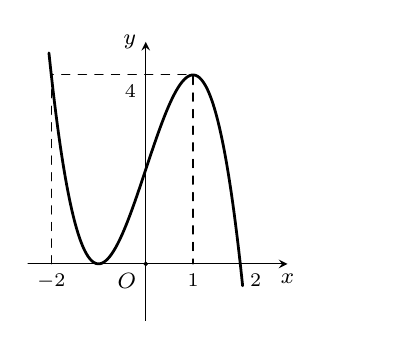
\begin{tikzpicture}[scale=0.6, font=\footnotesize, line join=round, line cap=round, >=stealth]
			\clip(-2.5,-1.2) rectangle (5,5);
			\draw[->] (-2.5,0) -- (3,0) node[below]{ $x$};
			\draw[->] (0,-1.5) -- (0,4.7) node[left]{ $y$};
			\draw[line width=1pt,smooth,samples=100,domain=-2.05:2.05] plot(\x,{-(\x)^3+3*(\x)+2});
			\draw [fill=black] (0,0) circle (1pt)node[below left]{\footnotesize $O$}(-1,1);
			\draw[dashed](-2,0)node[below]{\scriptsize $-2$}--(-2,4)--(0,4)node[below left]{\scriptsize $4$}--(1,4)--(1,0)node[below]{\scriptsize $1$};
			\draw(2,0)node[below right]{\scriptsize $2$};
	\end{tikzpicture}}
	
	\loigiai{
		Quan sát đồ thị, ta thấy nhánh cuối của đồ thị hướng xuống dưới nên $\lim\limits_{x\rightarrow +\infty}y=-\infty$, suy ra hệ số $a<0$. Như vậy hai hàm số 	$y=x^3+3x-2; y=x^3-3x+2$ không thỏa mãn.
		\\Mặt khác hàm số có hai điểm cực trị nên hàm số $y=-x^3-3x-2$ có $y'=-3x^2-3<0$ $\forall x\in \mathbb{R}$ không thỏa mãn.
	}
\end{ex} \dongcham{1}


\begin{ex}
	\immini[thm]{
		Đường cong bên là đồ thị của một trong bốn hàm số đã cho sau đây. Hỏi đó là hàm số nào?
		\choice
		{$y= - x^3 + 3x^2 + 1$}
		{$y= - x^2 - 3x - 1$}
		{$y=x^4 + 2x^2 - 1$}
		{\True $y=x^3 - 3x + 1$}
	}{
		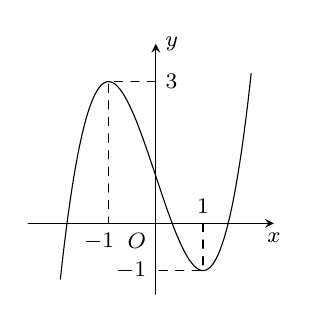
\begin{tikzpicture}[scale=0.6, font=\footnotesize, line join=round, line cap=round, >=stealth]
			\draw[->] (-2.7,0)--(0,0) node[below left]{$O$}--(2.5,0) node[below]{$x$};
			\draw[->] (0,-1.5) --(0,3.8) node[right]{$y$};
			\tkzDefPoints{0/0/O}
			\draw(-1.2,0) node[below]{$-1$};
			\draw(1,0) node[above]{$1$};
			\draw(0,-1) node[left]{$-1$};
			\draw(0,3) node[right]{$3$};
			\draw [domain=-2.02:2.02, samples=100] %
			plot (\x, {(\x)^3-3*(\x)+1}) ;
			\draw [dashed] (0,3)--(-1,3)--(-1,0);
			\draw [dashed] (1,0)--(1,-1)--(0,-1);
			\tkzDrawPoints[fill=black](O)
		\end{tikzpicture}
	}
	\loigiai{
		Đường cong trong hình là đồ thị của hàm số bậc ba có hệ số $a<0$. Trong các hàm số đã cho, chỉ có duy nhất hàm số $y=x^3 - 3x + 1$ thỏa mãn.
	}
\end{ex} \dongcham{1}

\begin{ex}
	\immini[thm]{Đường cong bên là đồ thị của một trong bốn hàm số đã cho sau đây. Hỏi đó là hàm số nào?
		\choice
		{$y=x^3-3x^2-4$}
		{$y=-x^3-4$}
		{$y=-x^3+3x^2-2$}
		{\True $y=-x^3+3x^2-4$}
	}{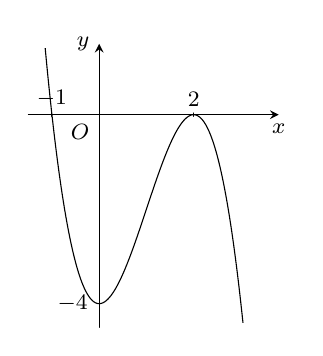
\begin{tikzpicture}[scale=0.6,>=stealth, font=\footnotesize, line join=round, line cap=round]
			\def\a{-1} \def\b{3} \def\c{0} \def\d{-4} % Hệ số
			\def\xmin{-1.5} \def\xmax{3.8}
			\def\ymin{-4.5} \def\ymax{1.5}
			%\draw[color=gray!50,dashed] (\xmin,\ymin) grid (\xmax,\ymax);
			\foreach \x in {-1,2}
			\draw[thin] (\x,1pt)--(\x,-1pt) node [above] {$\x$};
			\foreach \y in {-4}
			\draw[thin] (1pt,\y)--(-1pt,\y) node [left] {$\y$};
			\draw[->] (\xmin,0)--(\xmax,0) node [below]{$x$};
			\draw[->] (0,\ymin)--(0,\ymax) node [left]{$y$};
			\node at (0,0) [below left]{$O$};
			\clip (\xmin+0.1,\ymin+0.1) rectangle (\xmax-0.5,\ymax-0.1);
			\draw[smooth,samples=300] plot(\x,{\a*(\x)^3+\b*(\x)^2+\c*(\x)+\d});
	\end{tikzpicture}}
	\loigiai{
		\begin{itemize}
			\item Đồ thị hàm số có dạng chữ N ngược nên đây là đồ thị hàm số $y=ax^3+bx^2+cx+d$ với $a<0$. Loại phương án $y=x^3-3x^2-4$.
			\item Đồ thị hàm số giao $Oy$ tại điểm có tung độ bằng $-4$ nên $d=-4$, loại phương án $y=-x^3+3x^2-2$.
			\item Hàm số có hai điểm cực trị $x=0, x=2$ nên loại phương án $y=-x^3-4$ (vì phương án này có $y'=-3x^2$, hàm số không có điểm cực trị).
	\end{itemize}}
\end{ex} \dongcham{1}

\begin{ex}
	\immini[thm]{Đường cong bên là đồ thị của một trong bốn hàm số đã cho sau đây. Hỏi đó là hàm số nào?
		\haicot
		{$y=x^3-1$}
		{$y=(x+1)^3$}
		{\True $y=(x-1)^3$}
		{$y=x^3+1$}}
	{
		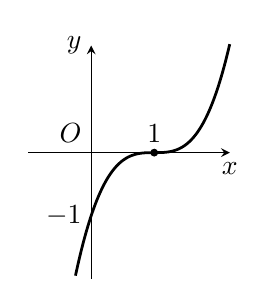
\begin{tikzpicture}[scale=0.8,>=stealth]
			\draw[->] (-1,0)--(0,0)node[above left]{$O$}--(2.2,0)node[below]{$x$};
			\draw[->] (0,-2)--(0,1.7)node[left]{$y$};
			\draw[line width=1pt,smooth,samples=100,domain=-0.25:2.2] plot(\x,{(\x-1)^3});
			\draw [fill=black] (1,0) circle (1.5pt);
			\draw (1,0)node[above]{$1$} (0,-1)node[left]{$-1$};
		\end{tikzpicture}
	}
	\loigiai{
		$(C)$ tiếp xúc với $Ox$ tại điểm uốn, suy ra $f(x)$ có nghiệm bội ba $x=1$ nên hàm số có dạng $y=a(x-1)^3$. Mà $(0;-1)\in (C)$ nên $a=1$.
	}
\end{ex} \dongcham{1}

\begin{ex}
	\immini[thm]{Cho hàm số $y = ax^3 + bx^2 + cx + d$ có đồ thị như hình vẽ bên. Khẳng định nào sau đây là đúng?
		
		\choice
		{$a > 0$, $b > 0$, $c > 0$, $d > 0$}
		{$a < 0$, $b < 0$, $c > 0$, $d > 0$}
		{$a > 0$, $b < 0$, $c < 0$, $d > 0$}
		{\True $a > 0$, $b < 0$, $c > 0$, $d > 0$}}
	{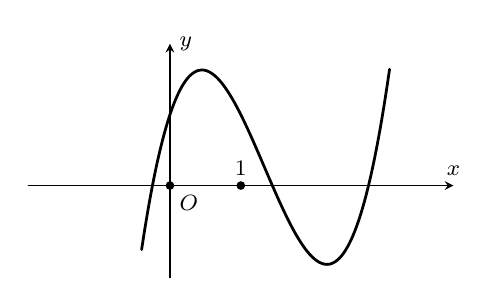
\begin{tikzpicture}[scale=0.9, font= \footnotesize, line join=round, line cap=round, >=stealth]
			\draw[->] (-2,0) -- (4,0) node[above] {$x$};
			\draw[->] (0,-1.3) -- (0,2) node[right] {$y$};
			\draw[fill=black] (1,0) circle (1.5pt);
			\draw[fill=black] (0,0) circle (1.5pt);
			\draw[line width=1pt,smooth,samples=100,domain=-0.4:3.1] plot(\x,{(\x)^3-4*(\x)^2 + 3*(\x) + 1});
			\node[below right] at (0,0) {$O$};
			\node[above] at (1,0) {$1$};
	\end{tikzpicture}}
	
	\loigiai{
		Nhìn vào đồ thị, ta thấy đồ thị hàm số đi từ $-\infty$ lên $+\infty$ nên $a > 0$. \\
		Giao điểm với trục tung nằm trên trục hoành, do đó $d > 0$.\\
		Hàm số có hai điểm cực trị, và hai điểm cực trị đều dương. Suy ra tổng hai điểm cực trị và tích hai điểm cực trị đều dương.\\ 	Ta có $f'(x) = 3ax^2 + 2bx + c$ nên tổng hai điểm cực trị là $\dfrac{-2b}{3a}$. Suy ra $\dfrac{-2b}{3a} > 0$, hay $b < 0$.\\ Còn tích hai điểm cực trị là $\dfrac{c}{3a}$. Suy ra $\dfrac{c}{3a} > 0$ hay $c > 0$.}
\end{ex} \dongcham{1}

\begin{ex}%[2D1B5-1]
	\immini[thm]{Cho hàm số $ y=ax^3+bx^2+cx+d $ có đồ thị như hình vẽ bên. Mệnh đề nào sau đây đúng?
		\choice
		{$ a<0 $, $ b<0 $, $ c<0 $, $ d>0 $}
		{$ a<0 $, $ b>0 $, $ c<0 $, $ d>0 $}
		{\True $ a<0 $, $ b>0 $, $ c>0 $, $ d<0 $}
		{$ a<0 $, $ b<0 $, $ c>0 $, $ d<0 $}}{
		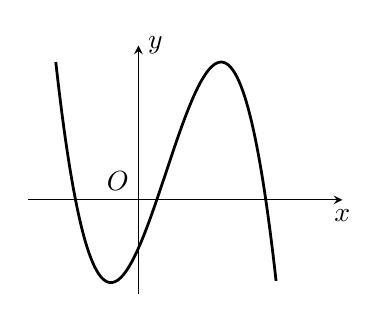
\begin{tikzpicture}[smooth,samples=300,scale=0.7,>=stealth]
			\draw[->] (-2,0)--(3.7,0) node[below]{$x$};
			\draw[->] (0,-1.7)--(0,2.8) node[right]{$y$};
			\draw (0,0) node[above left]{$O$};
			\draw[line width=1pt,domain=-1.5:2.5] plot(\x,{-(\x-0.5)^3+3*(\x-0.5)+0.5});
		\end{tikzpicture}
	}
	\loigiai{
		Dựa vào hình dáng đồ thị suy ra $ a<0 $.\\
		Dựa vào vị trí điểm cực đại và điểm cực tiểu, suy ra $ x_{\text{CT}}+x_{\text{CĐ}}>0 \Rightarrow -\dfrac{b}{a}>0\Rightarrow b>0$.\\
		Hai điểm cực trị có hoành độ trái dấu nên $ x_{\text{CT}}\cdot x_{\text{CĐ}}<0\Rightarrow \dfrac{c}{a}<0\Rightarrow c>0 $.\\
		Đồ thị hàm số cắt trục tung tại điểm có tung độ dương nên $ d>0 $.\\
		Vậy $ a<0 $, $ b>0 $, $ c>0 $ và $ d>0 $.
	}
\end{ex} \dongcham{1}

\begin{ex}%[2D1K5-1]
	\immini[thm]{Cho hàm số $y=ax^3+bx^2+cx+d$ có đồ thị như hình vẽ bên. Mệnh đề nào dưới đây đúng?
		\choice
		{$a<0$, $b>0$, $c>0$, $d>0$}
		{$a<0$, $b<0$, $c=0$, $d>0$}
		{\True $a<0$, $b>0$, $c=0$, $d>0$}
		{$a>0$, $b<0$, $c>0$, $d>0$}}{
		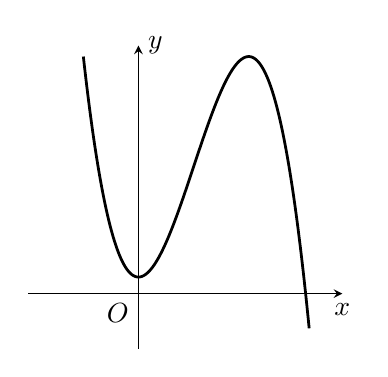
\begin{tikzpicture}[smooth,samples=300,scale=0.7,>=stealth]
			\draw[->] (-2,0)--(3.7,0) node[below]{$x$};
			\draw[->] (0,-1)--(0,4.5) node[right]{$y$};
			\draw (0,0) node[below left]{$O$};
			\draw[line width=1pt,domain=-1:3.1] plot(\x,{-(\x)^3+3*(\x)^2+0.3});
			%\draw[fill=black] (2,-1) circle(1.5pt) (2,0) circle(1pt) (0,-1) circle(1pt);
			%\draw[dashed] (2,-1.5)--(2,2.5) (2,-1)--(0,-1)node[left]{\small$-\dfrac{\Delta}{4a}$};
			%\node[right] at (2,2.4) {\small $x=-\tfrac{b}{2a}$};
			%\node[right] at (0.5,-2) {\fbox{$a>0$}};
		\end{tikzpicture}
	}
	\loigiai{
		Dựa vào đồ thị ta có thể thấy $a<0$, đồ thị cắt trục tung tại điểm có tung độ dương nên $d>0$.\\
		Hàm số có hai cực trị thỏa $\heva{&S>0\\&P=0}\Leftrightarrow\heva{&-\dfrac{b}{a}>0\\&\dfrac{c}{a}=0}\Leftrightarrow\heva{&b>0\\&c=0.}$
	}
\end{ex} \dongcham{4}

\begin{ex}
	\immini[thm]{Cho hàm số $y=ax^3+bx^2+cx+d$ có bảng biến
	thiên như hình bên. Trong các hệ số $a$, $b$, $c$ và $d$ có bao nhiêu số âm?
	\choice
	{$2$}
	{\True $1$}
	{$4$}
	{$3$}}{

\begin{tikzpicture}[>=stealth,scale=1]
	\tkzTabInit[lgt=1.2,espcl=2]
	{$x$ /0.6, $f’(x)$ /0.6, $f(x)$ /2}
	{$-\infty$,$-1$,$2$,$+\infty$}
	\tkzTabLine{ ,-,z,+,z,-, }
	\tkzTabVar{+/,-/$0$,+/,-/}
\end{tikzpicture}}
	\loigiai
	{
		Từ bảng biến thiên ta thấy hàm số có $2$ điểm cực trị nên bậc của đa thức phải lớn hơn $2\Rightarrow a\ne 0$. Mà $\lim \limits_{x \to +\infty} y=-\infty\Rightarrow a<0$.\\
		Từ bảng biến thiên ta có $d=y(0)>y(-1)=0$.\\
		Ta có $y'=3ax^2+2bx+c$ có hai nghiệm là $-1$ và $2$ nên $\heva{& -\dfrac{2b}{3a}=-1+2=1>0 \\ & \dfrac{c}{3a}=(-1)\cdot 2=-2<0}\Rightarrow \heva{& b>0 \\ & c>0.}$
	}
\end{ex} \dongcham{4}

\Closesolutionfile{ans}

\ind{PHẦN II.} \inden{Câu trắc nghiệm đúng sai. Trong mỗi ý a), b), c), d) ở mỗi câu, học sinh chọn đúng hoặc sai.}\\
\Opensolutionfile{ans}[ans/2D1-B4-d1-2]

\begin{ex}
	\immini[thm]{Cho hàm số $y=f(x)=ax^3+bx^2+cx+d$ có đồ thị như hình vẽ.
		\choiceTF
		{Hàm số đạt cực tiểu tại $x=1$}
		{\True Đồ thị hàm số cắt trục $Oy$ tại điểm $(0;1)$}
		{Hàm số đồng biến trên khoảng $(-\infty;-1)$}
		{$2a+3b+c=9$}
	}{
		\begin{tikzpicture}
			[scale=1,line join=round, line cap=round, >=stealth]
			\draw[->] (-3,0)--(0,0) node[below left]{$O$}--(2,0) node[below]{$x$};
			\draw[->] (0,-1) --(0,3) node[right]{$y$};
			\draw [domain=-2.3:.7, samples=100] %
			plot (\x, {(\x)^3+2*(\x)^2+1});
			\draw [dashed] (-2,0)node[below]{$-2$}--(-2,1) --(0,1)node[below right]{$1$}
			(-1,0)node[below]{$-1$}--(-1,2)--(0,2)node[right]{$2$};
			\draw[fill] (0,1) circle (1pt) (-2,1) circle (1pt) (-1,2) circle (1pt);
		\end{tikzpicture}}
	\loigiai{
		Theo hình vẽ thì:
		\begin{enumerate}[a)]
			\item Hàm số đạt cực tiểu tại $x=0$, giá trị cực tiểu $y=1$;
			\item Đồ thị hàm số cắt trục $Oy$ tại điểm $(0;1)$;
			\item Hàm số đồng biến trên khoảng $(-\infty;x_0)$, với $-2<x_0<-1$;
			\item Đồ thị qua 3 điểm $(-2;1)$, $(-1;2)$, $(0;1)$ và đạt cực trị tại $x=1$ nên ta được hệ
			$$\heva{&-8a+4b-2c+d=1\\&-a+b-c+d=2 \\& d=1\\&c=0} \Leftrightarrow a=1;\,b=2,\,c=0,\,d=1$$
			nên $2a+3b+c=8$.
		\end{enumerate}
	}
\end{ex} \dongcham{10}

\begin{ex}
	\immini[thm]{Cho hàm số bậc ba $ f(x)=ax^3+bx^2+cx+d $ có đồ thị như hình vẽ.\\
		Tính tổng $ T=$.
		\choiceTF
		{\True Đồ thị hàm số cắt trục tung tại điểm $(0;1)$}
		{\True Đường thẳng đi qua điểm $(0;1)$ luôn cắt đồ thị tại ba điểm phân biệt có hoành độ lập thành 1 cấp số cộng}
		{\True $a-b+c+d =-1$}
		{Đồ thị hàm số đi qua điểm $(3;18)$}
	}{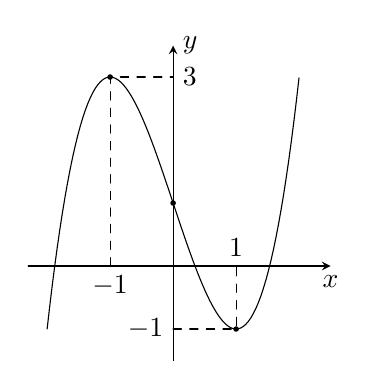
\begin{tikzpicture}[>=stealth,line join=round,line cap=round,scale=.8]
			\draw[->] (-2.3,0)--(2.5,0)node[below]{$x$};
			\draw[->] (0,-1.5)--(0,3.5)node[right]{$y$};
			\draw[domain=-2:2, samples=100] plot (\x,{(\x)^3-3*(\x)+1});
			\draw[fill] (-1,3) circle (1pt) (0,1) circle (1pt) (1,-1) circle (1pt);
			\draw[dashed] (-1,0)node[below]{$-1$}|-(0,3)node[right]{$3$} (0,-1)node[left]{$-1$}-|(1,0)node[above]{$1$}
			;
	\end{tikzpicture}}
	\loigiai{
		\begin{enumerate}[a)]
			\item Đồ thị hàm số có hai điểm cực trị $(-1;3)$ và $(1;-1)$. Suy ra tọa độ tâm đối xứng là $(0;1)$. Suy ra đồ thị hàm số cắt trục tung tại điểm $(0;1)$
			\item Do $I(0;1)$ là tâm đối xứng của đồ thị, nên đường thẳng qua nó sẽ cắt đồ thị tại ba điểm phân biệt $I$, $A$, $B$ với $I$ là trung điểm của $AB$. Suy ra $x_A+x_B=2x_I$. Vậy ba điểm này có hoành độ lập thành 1 cấp số cộng.
			\item Ta có $ f'(x)=3ax^2+2bx+c $. Từ hình vẽ, ta có
			$$\heva{&f(-1)=3\\&f(1)=-1\\&f'(-1)=0\\&f'(1)=0} \Leftrightarrow \heva{&-a+b-c+d=3\\&a+b+c+d=-1\\&3a-2b+c=0\\&3a+2b+c=0}$$
			Giải hệ, ta được $a=1$, $b=0$, $c=-3$,$d=1$.
			Vậy $ T=a-b+c+d=-1 $.
			\item Ta có $ f'(x)=3ax^2+2bx+c $. Từ hình vẽ, ta có
			$$\heva{&f(-1)=3\\&f(1)=-1\\&f'(-1)=0\\&f'(1)=0} \Leftrightarrow \heva{&-a+b-c+d=3\\&a+b+c+d=-1\\&3a-2b+c=0\\&3a+2b+c=0}$$
			Giải hệ, ta được $a=1$, $b=0$, $c=-3$,$d=1$. Suy ra $y=x^2-3x+1$.\\
			Thay tọa độ $(3;18)$ vào phương trình, không thỏa mãn. Vậy đồ thị hàm số không đi qua điểm $(3;18)$.
		\end{enumerate}
		}
\end{ex} \dongcham{14}

\begin{ex}
	\immini[thm]{Cho hàm số $ y=f(x)=ax^3+bx^2+cx+d$ có bảng biến thiên như hình bên.
		\choiceTF
		{Hàm số đạt giá trị lớn nhất là $ 4 $}
		{\True Đường thẳng $ y=2$ cắt đồ thị hàm số $ y=f(x)$ tại $ 3 $ điểm phân biệt}
		{\True Trong bốn hệ số $a$, $b$, $c$, $d$ có đúng hai số âm}
		{\True Đồ thị hàm số đi qua điểm $(-4;20)$}
	}{
		
\begin{tikzpicture}
			\tkzTabInit[nocadre=false,lgt=1.2,espcl=1.6,deltacl=0.6]
			{$x$ /0.6, $y'$ /0.6, $y$ /2.3}
			{$-\infty$,$-2$,$0$,$+\infty$}
			\tkzTabLine{,-,0,+,0,-,}
			\tkzTabVar{+/$+\infty$,-/$0$,+/$4$,-/$-\infty$}
	\end{tikzpicture}}
	\loigiai{
		Dựa vào bảng biến thiên ta thấy:
		\begin{enumerate}[a)]
			\item Hàm số $ y=f(x)$ không có giá trị lớn nhất trên $\mathbb{R}$.
			\item Vẽ đường thẳng $y=2$ qua điểm $(0;2)$ và song song với $Ox$, rõ ràng đường thẳng này cắt đồ thị tại ba điểm phân biệt.
			\item Từ các thông số trên hình, ta có thể giải ra chính xác giá trị $a$, $b$, $c$, $d$ bởi hệ
			$$\heva{&f(-2)=0\\&f(0)=4\\&f'(-2)=0\\&f'(0)=0} \Leftrightarrow a=-1,\,b=-3,\,c=0,\,d=4.$$
			Vậy trong 4 hệ số, có đúng 2 số âm.
			\item Từ các thông số trên hình, ta có thể giải ra chính xác giá trị $a$, $b$, $c$, $d$ bởi hệ
			$$\heva{&f(-2)=0\\&f(0)=4\\&f'(-2)=0\\&f'(0)=0} \Leftrightarrow a=-1,\,b=-3,\,c=0,\,d=4.$$
			Suy ra $y=-x^3-3x^2+4$. Thay tọa độ $(-4;20)$ vào phương trình, thỏa mãn. Suy ra Đồ thị hàm số đi qua điểm $(-4;20)$.
		\end{enumerate}
		
	}
\end{ex} \dongcham{14}

\Closesolutionfile{ans}




